\section{Security Models for Verifiable DP}
\label{sec:model}

%\begin{figure}[t]
%    \centering    
%	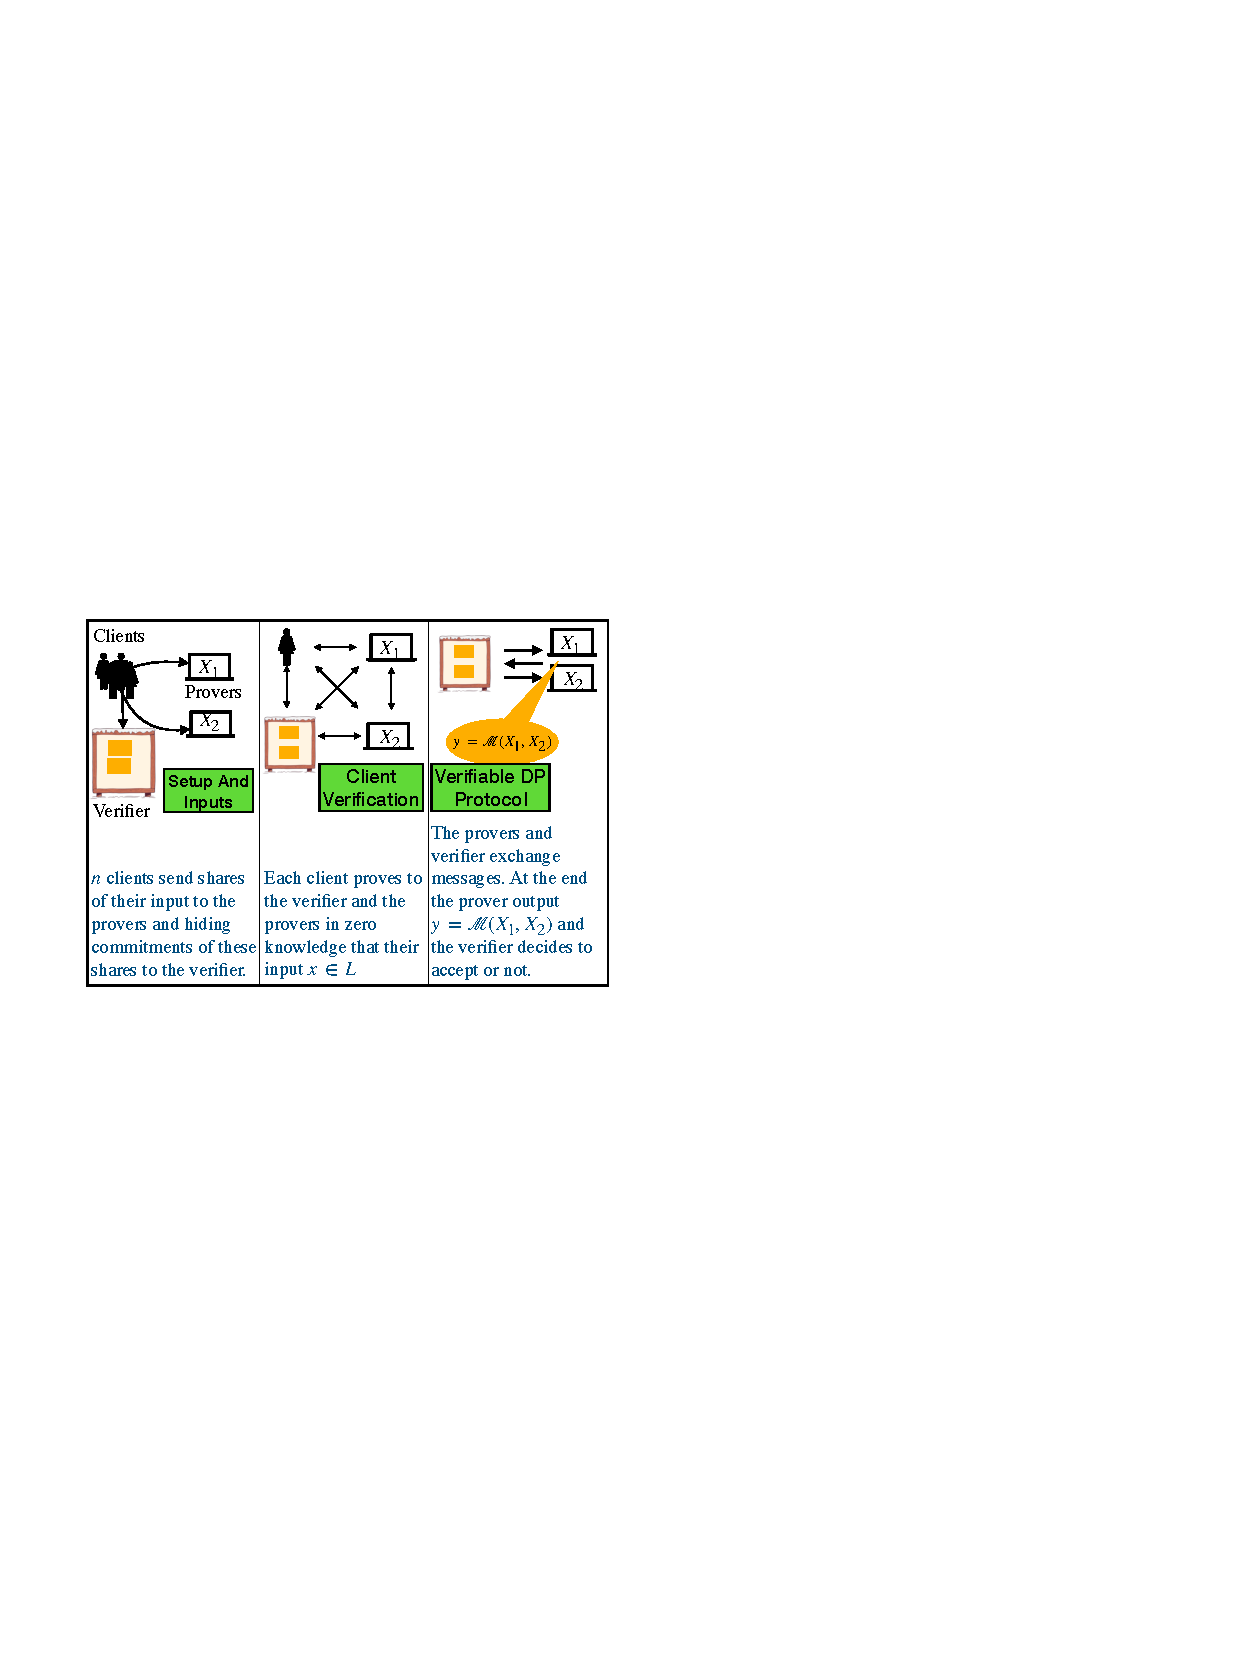
\includegraphics[scale=0.9]{pngs/data_flow.pdf}
%	\caption{The figure above describes the three stages of the protocol.  Any message sent and received by the verifier is accessible to all clients and provers. In the setup stage, public parameters are generated, and each client $i \in [n]$ sends inputs to the prover and the verifier.  In the verification stage, each client interactively exchanges messages with the verifier and the provers to establish their private input $x \in L$ in zero knowledge. If a client fails to do so, they are tagged as dishonest and excluded from the protocol. In the last stage, each prover samples private randomness and then interactively exchanges messages with other provers and the verifier to jointly compute $y = \mathcal{M}_Q(X_1, \dots, X_K)$ for some common knowledge query $Q$.
%	The verifier validates that the provers' output $y$ was computed as prescribed over the inputs of honest clients only. }
%	\label{fig:flow}
%\end{figure}


This section introduces definitions for interactive proofs for differential privacy. The definitions apply to both the single curator and MPC setting.
In both settings, we will assume that the inputs comes from $n$ distinct clients.
Informally, the main difference between the two
models is that the single curator has plaintext access to the client data $X = (x_1, \dots, x_n)$. 
In contrast, in MPC-DP, the client's secret share (or partition) their inputs and each server receives information theoretically hiding shares (or a partial view) of client inputs. 
Additionally, for a given query $f \in \FuncFamily$, instead of having a single entity responsible for outputting samples from $\Mechanism(X, f)$, the servers participate in an MPC protocol denoted by $\Pi$ to securely sample from $\Mechanism(X, f)$.
For some queries $f \in \FuncFamily$, the specifications may require that the client inputs come from a restricted subset $L \subseteq \FuncDomain$.
For such cases, the clients must prove in zero-knowledge to an independent verifier that their inputs come from the specified language without revealing any other information about their inputs. Going back to our pizza topping example in Section \ref{sec:introduction}, the client must prove that they voted for at most one option at most one time.  
Examples of such proofs can be found in the prior literature~\cite{boneh_lightweight_2022,
  boyle2019secure, corrigan-gibbs_prio_2017, bunz2018bulletproofs}.
In the definitions below and in what follows, we use the terms $\Prover$
(prover), server and curator interchangeably, and the terms analyst and
$\Verifier$ (verifier) to refer to the same entity. Unless otherwise specified, for $K \geq 1$, it is safe to assume that the provers $\vec{\Prover} = (\Prover_1, \dots, \Prover_K)$ and verifier $\Verifier$ are PPT Turing Machines.

%\input{tex_files/single_curator_dp_defs.tex}
\subsection{Verifiable DP}

\paragraph{MPC Model}
Next, we describe the MPC model and later discuss how the single curator model is a special case of the general model.
Let $\Mechanism$ be a DP (or IND-CDP) mechanism as described in Definition~\ref{def:dp_approx_definition} (or Definition~\ref{def:comp_dp_definitions} respectively) for a query $f$.  
Let $\SecurityParam \in \Naturals$ denote the security parameter and $n=\lceil\poly(\SecurityParam)\rceil$ denote the number of inputs to the DP mechanism. Let $K \geq 1$ denote the number of provers. A verifiable DP mechanism for $\Mechanism$  consists of a PPT algorithm $\Setup$  and an interactive proof system $\Pi$, between $K+1$ ``next-message-computing-turing machines'' $\Verifier$ and $(\Prover_1, \dots, \Prover_K)$. 
In next-message computing-turing machines, any party, for example, $\Verifier$'s message $m_i$ at round $i$ is determined by its input, messages it has received so far from other parties and internal randomness $\vec{r}_\Verifier$.  
Let $\vec{\Prover}$ denote a succinct representation for $(\Prover_1, \dots, \Prover_K)$. 
$\pp \samples \Setup(1^\SecurityParam)$ describes the PPT algorithm that receives a unary representation of the security parameter $\SecurityParam$ as input and generates public parameters $\pp$ that are broadcasted to all parties.

$\Pi$ describes a multi-prover interactive proof system for differential privacy between $K$ provers and a single verifier. In a multi-prover interactive proof system, the provers and verifier exchange messages for $\poly(\SecurityParam)$ rounds. Let $z \in \bit^{\poly(\SecurityParam)}$ denote auxiliary input available to the verifier $\Verifier$. In a specific rounds\footnote{These rounds need not be the last round of the proof. A proof system may prescribe that the prover send a message tagged as the output and continue to exchange messages in future rounds.} of message exchanging, each prover $\Prover_j$ sends to the verifier $\Verifier$ special messages $y_j$ tagged as the output. Once the verifier has received output messages from every prover, it uses a pre-specified deterministic polynomial time algorithm $A$ to compute $y = A(y_1, \dots, y_k)$. As for all $j \in [K]$, $y_j$ is computed as a function of $\Prover_j$'s internal randomness, $y$ can be viewed as a random sample from the distribution $\Pi(\Verifier, \vec{\Prover}) \in \Delta(\FuncRange)$. Once all messages have been exchanged, the verifier $\Verifier$,  outputs either 0 or 1, with 1 indicating that the verifier accepts the provers' claim that $\Mechanism(X, f)=\Pi(\Verifier, \vec{\Prover})$ and $y$ is a sample from $\Mechanism(X, f)$, and 0 indicating otherwise.

Let $\Output\Big[\Verifier(\pp, \vec{r}_\Verifier, z), \vec{y}, \vec{\Prover}(X, \pp, \vec{r}_{\vec{\Prover}})\Big] \in \bit$ denote the verifying algorithm's decision.
In the definition below, we write $\Output(\Verifier, \Prover)$ as shorthand for the verifier output.
%In $\texttt{Setup}$, all parties jointly generate public parameters and the provers and verifier receives inputs from $n$ clients. 
%Let $ \texttt{Setup}(1^\SecurityParam)$ denote public parameters. 
%Each prover $\Prover_k$ receives on its input tape $n$ secret shares of client inputs $\Big(\share{x_1}_k, \dots, \share{x_n}_k\Big)$, succinctly denoted by $\vec{X_k}$.
%The verifier receives hiding commitments of the above shares. All messages sent and received by the verifier are accessible to all other parties. \par
If the query $f$ restricts client inputs to a subset $L \subseteq \mathcal{X}$ then in $\texttt{Verify}$ phase, the clients interactively exchange messages with the provers and the verifier to prove in zero knowledge that their private input $x \in L$. If clients fail to do so, they are excluded from the protocol. 
Once dishonest clients with illegal inputs have been excluded and honest client inputs have been recorded, the clients play no further role in the protocol. \par



\paragraph{Single Curator}
The single curator can be understood as
essentially the above model with a single prover, i.e., we set $K=1$.  Thus
the only functional difference between MPC-DP and trusted curator DP
is that in the latter case, the curator sees all client inputs in plaintext. 
In MPC, the data may be secret, shared or partitioned
across the provers. 
In both cases, the prover(s) must prove they did not tamper with the protocol to sample an output from a distribution that is different from that specified by $\Mechanism$ \footnote{When there is a single server only, and the client inputs come from a restricted set $L$, although the server can see inputs in plaintext, the verifier cannot. Thus, to prevent malicious clients from colluding with the server, the clients still need to prove to the verifier with zero-knowledge that the inputs are legal.}. Figure \ref{fig:flow} summarises the information flow between the parties.

\statetheoremsolid{0.95\textwidth}{
\begin{definition}[Interactive Proofs For DP]\label{defn:vdp_MPC}
 Fix $\SecurityParam \in \Naturals$ as the security parameter. Let $\Mechanism$ be a DP (or CDP) mechanism for computing $f$ using inputs $X=(x_1, \dots, x_n)$ received from $n$ distinct clients (input sources). Let $K \geq 1$ and $(X_1, \dots, X_K)$ denote a partitioning/secret sharing of $X$ such that there exists a public deterministic PPT reconstruction algorithm $A$, such that $X = A(X_1, \dots, X_K)$.  An interactive proof for verifying $\Mechanism$ consists of a PPT algorithm $\Setup$ and a multi-prover (single if $K=1$) interactive proof system $\Pi$. $\pp \samples \Setup(1^\SecurityParam)$ describes the PPT algorithm that receives a unary representation of the security parameter as input and generates public parameters $\pp$. $\Pi$ denotes a multi prover interactive proof system between, $K \geq 1$ provers $\vec{\Prover}=(\Prover_1, \dots, \Prover_K)$ and a single verifier $\Verifier$ where for each $j \in [K]$, $(X_j, \vec{r_{\Prover_j}}, \pp)$ denotes the inputs for $\Prover_j$ and $(\vec{z}, \vec{r}_\Verifier, \pp)$ denote the verifiers input. Here where $\vec{r_{\Prover_j}}$ and $\vec{r_{\Verifier}}$ denotes $\Prover_j$'s and the verifiers internal randomness respectively and $\vec{z}$ denotes the verifiers auxiliary input. The proof system $\Pi$ is an interactive proof system for mechanism $\Mechanism$ if there exists negligible functions $\delta_c$ and $\delta_s$ in $\SecurityParam$ such that the following hold:

\begin{enumerate}
\item{\textbf{Completeness:} Let $\Pi(\vec{\Prover}, \Verifier)$ denotes the induced output distribution from which the verifier samples the final output $y \samples \Pi(\vec{\Prover}, \Verifier)$ if the verifier and all provers are honest. If $\TV{(\Pi(\vec{\Prover}, \Verifier) , \Mechanism(X, Q))} =0$

    
     \[ \Pr\left[ \texttt{out}(\Verifier, \vec{\Prover}) = 0 : \begin{array}{c} \pp \samples \texttt{Setup}(1^\kappa) \\
      \Prover_j \gets (X_k, \vec{r}_{\Prover_j}, \pp)\\
     \Verifier \gets (\vec{z}, \vec{r}_\Verifier, \pp) \\
y \samples \Pi(\vec{\Prover}, \Verifier) 
    \end{array} \right]
  \leq \delta_c . \] 
  }

\item{\textbf{Soundness:} For any
    subset, $I \subseteq [K]$, let $\vec{\ChProver}$ denote the collection
    of corrupted provers, indexed by $I$,  that deviate from $\Pi$, and $\vec{\Prover}$  denote the set of honest provers not indexed by $I$. Let $\Pi(\vec{\Prover}, \vec{\ChProver}, \Verifier)$ denote the induced output distribution from which the verifier samples the final output $y \samples \Pi(\vec{\Prover}, \vec{\ChProver}, \Verifier)$. Then, if $\TV{(\Pi(\vec{\Prover}, \vec{\ChProver}, \Verifier), \Mechanism(X, Q))} >0$

     \[ \Pr\left[ \texttt{out}(\Verifier,\vec{\Prover}, \vec{\ChProver}) = 1 : \begin{array}{c} \pp \samples \texttt{Setup}(1^\kappa) \\
      \Prover_j \gets (X_k, \vec{r}_{\Prover_j}, \pp)\\
     \Verifier \gets (\vec{z}, \vec{r}_\Verifier, \pp) \\
y \samples \Pi(\vec{\Prover}, \vec{\ChProver}, \Verifier)
    \end{array} \right]
  \leq \delta_s . \] 
  
\ariInline{There is room for interactive proofs for proximity here. Talk to Graham or Vadhan.}  

}
     
\item{\textbf{Zero Knowledge}:  Let $\ChVerifier$ denote an arbitrary verifier strategy that corrupts any proper subset $I \subset [K]$ of provers. 
Let $\vec{\ChProver}$ denote the collection of corrupted provers, indexed by $I$, and $\vec{\Prover}$  denote the set of honest provers.  Let
    $\View\Big[\Pi\Big((\vec{\Prover}, \vec{\ChProver})
    ,\ChVerifier\Big)\Big]$ be the joint distribution\footnote{As
      $\Mechanism$ is a random function, the \highlight{joint
        distribution} of the view of the adversary and \highlight{their output}
      must be indistinguishable from the simulated transcript (and not
      just the view of the adversary). See \cite{lindell2017simulate}
      for more details.} of exchanged messages and induced output distribution $\Dist$ during the
    execution of $\Pi$ in the presence of corrupted parties. There
    exists a PPT algorithm called $\Simulator^{(\ChVerifier, \vec{\ChProver}, \Dist)}$ with black box access to $\ChVerifier$ and $\vec{\ChProver}$ and sample access to $\Dist$, such that if $\TV{(\Dist, \Mechanism(X, Q))}=0$
    
    
    \begin{align*}
\View\Big[\Pi\Big((\vec{\Prover}, \vec{\ChProver})
    ,\ChVerifier\Big)\Big] &\stackrel{}{\equiv} \Simulator^{(\ChVerifier, \vec{\ChProver}, \Dist)}(\vec{r}_\Verifier, \vec{z})        
    \end{align*}
 }

\end{enumerate}
 \end{definition}
}

 Verifiable DP, just like interactive zero knowledge proofs \cite{goldreich_foundations_2007} comes in 24 different flavours based on the capabilities of the corrupted parties:
 
 \begin{enumerate}
 	\item{\textbf{Distinguishability:} Based on the distinguishability properties of the simulator algorithm, the protocol may be perfect, statistical or computationally zero knowledge. The protocol described in Section \ref{sec:single_curator_hist} is computationally zero knowledge. } 
 	\item{\textbf{Verifier specifications:} Based on whether the verifier is expected to follow the rules of the protocol (semi-honest) or may deviate arbitrarily (active), we get honest-verifier zero knowledge or malicious verifier zero knowledge. All our results are malicious verifier zero knowledge.}  	
 	\item{\textbf{Soundness:} Based on the power of the corrupted provers, the proof may be computationally sound (also known as arguments) or statistically sound (secure against unbounded provers). The verifiable DP protocol in Section \ref{sec:single_curator_hist} is computationally sound.}  	
 	\item{\textbf{Inputs:} Based on whether the verifier has access to the auxiliary input, the protocol could be plaintext zero knowledge or auxiliary input zero knowledge. Our protocols allow for the verifier to have auxiliary input.}  	 	
 \end{enumerate}

 
\begin{remark}
 Contrary to soundness, for zero knowledge to hold, the simulated transcript should be indistinguishable from the actual protocol transcript, based on the inputs adversaries used and not the ones the clients sent to a set of corrupted provers.	
\end{remark} 
 
 \begin{remark}
 An interesting point to note is that here verifier plays a dual role. An honest verifier ensures
 that the output is faithfully generated and thus plays an active role in noise generation without ever knowing the value of the random variable.	 On the other hand, a dishonest verifier tries to tamper with the protocol to breach privacy. 
  In non-verifiable DP, the analysts
 (verifier) only has sample access to the induced distribution. They have no agency over how this distribution is constructed. Thus the verifier
 participating in verifiable DP has a greater attack surface than a classical adversary in traditional non-verifiable DP. 
 We elaborate on this in Section \ref{sec:separation}, when trying to establish separations between statistical DP and computational DP.
 \end{remark}
 
 \begin{remark}
Just like in standard MPC, in the presence of a dishonest majority of corrupted participants, we do not treat early exiting by corrupted parties as a breach of security. This is easily detected by the honest parties, and the output is ignored. 	
 \end{remark}
 
